\chapter{Controllability and Observability}

\section{Stability of State-space systems}

In this section a formal definition of stability of systems in the context of state-space models are provided. Initially defining the equilibrium for a system, a core test to check if there exists an equilibrium point for a given system such that a state remains in this point once there and also (for stability) converges to that the point from anywhere near this neighborhood.

\subsection{Equilibrium}

In the most obvious definition for equilibrium is that the state dynamics are zero at the equilibrium point such that the derivative of the states are zero, which is as expressed:
\begin{equation}
	\dot{x} = 0 = Ax + Bu
\end{equation}
this follows the condition that the update of a state at the next instance is the same position of the state in the state configuration such that
\begin{equation}
	x_{k+1} = x_{k}
\end{equation}
which simply means that the states do not evolve. To arrive at the equilibrium point if the system also has inputs $u$ to it, then different values of $u$ will lead to different equilibrium points of the system. However, for the sake of simplicity, the control input $u$ at the equilibrium point is considered to be zero. As this is a LTI system, for any other values of $u$, the systems response can be super-imposed later.

\subsection{Stable Equilibrium}

A stable equilibrium is defined using \textbf{\textit{norms}} of a vector $\norm{x(t)}$ and establishes that once a state is within a certain distance from the equilibrium point, thereafter, that state will never go farther away from a certain relative distance. This definition does not allow for convergence but it does allow for the boundedness such as in the case of oscillations.

\textbf{\textit{Note: }} A norm of a vector defines the radial distance from the origin, in this case, the origin being the equilibrium point. Therefore, using norm the definition of state's equilibrium can be established.

Mathematically, stable equilibrium can be expressed as:
\begin{equation}
	\norm{x(t)} \leq \delta \implies \norm{x(t + t_{1})} \leq r \delta, \quad t > 0
\end{equation}
where $r$ is a scaling factor (radial position of the boundary $\delta$) to be determined for a given system. In case of \textbf{\textit{linear}} systems, $r$ is independent of the magnitude $x$. The above definitions allows for permanent oscillations without convergence.

\subsection{Asymptotic stability}

This case is similar to stable equilibrium with the difference that in this case the definition insists on convergence such that
\begin{equation}
	\lim_{t \to \infty} \norm{x(t)} = 0
\end{equation}
Therefore, by the definition, pure oscillation modes or sinusoids are not allowed if the system is to be defined asymptotically stable.

\subsection{BIBO}

This case is defined when using control inputs such that, assuming the inputs are bounded beneath some boundary value $\delta$, it can be guaranteed that the states are also beneath some boundary vale $\epsilon$. The boundary values just like in previous cases can be expressed using the norm of the vector.
\begin{equation}
	\norm{u(t)} \leq \delta, \forall t \geq 0 \implies \norm{x(t)} \leq \epsilon, \forall t \geq 0
\end{equation}
This definition now allows for system with an input to be within well defined boundary of equilibrium without being blown-up. In general, the norms may depend upon the initial condition, but for linear systems, one could make these relationships more precise if desired.

\textbf{\textit{Note: }}In general, for analyzing the stability of forced systems, BIBO definition is used and for analyzing stability of free systems, definition of Asymptotic stability is used.

\section{Defining controllabilty} \label{Sec_2_ch_25_Controllabiliry}

In this example a discrete system is considered because using a discrete system it would be fairly easier to define the idea of controllability of the system. In any case, the resulting solutions apply the same to continuous systems as well. 

Consider a linear discrete system given by,
\begin{equation}
	\vec{\dot{x}}_{k} = \vec{{A}}_{k} {x}_{k} + \vec{{B}}_{k} {u}_{k}
\end{equation}
at an initial condition $x_0 = 0$. If this system is completely controllable, such that it can be driven some arbitrary point $x^{*}$, then a map of all the states and control inputs can be made for each of the discrete step as following,
\begin{align*}
	\vec{{x}}_{1} &= \vec{{A}}_{0} {x}_{0} + \vec{{B}}_{0} {u}_{0} = \vec{{B}}_{0} {u}_{0} \\
	\vec{{x}}_{2} &= \vec{{A}}_{1} {x}_{1} + \vec{{B}}_{1} {u}_{1} = \vec{{A}} \vec{{B}}_{0} {u}_{0} + \vec{{B}}_{1} {u}_{1} \\
	\vec{{x}}_{3} &= \vec{{A}}_{2} {x}_{2} + \vec{{B}}_{2} {u}_{2} = \vec{{A}}^{2} \vec{{B}}_{0} {u}_{0} + \vec{{A}} \vec{{B}}_{1} {u}_{1} + \vec{{B}}_{2} {u}_{2} \\
\end{align*}
Performing the similar calculations up until $n^{th}$ iteration when $x$ reaches the final destination $x^{*}$,
\begin{equation}
	\vec{{x}}_{n} = \vec{A}^{n - 1} \vec{B}u_{0} + ... + \vec{B}u_{n - 1}
\end{equation}
therefore, in general it an be said that in order to reach a final point $x^{*}$, the linear controllable model can be expressed in matrix form as
\begin{equation}
	x^{*} = [\vec{B} \quad \vec{A}\vec{B} \quad ... \quad \vec{A}^{n - 1} \vec{B}]\begin{bmatrix}
		u_{n - 1} \\ . \\. \\. \\ u_{1} \\ u_{0}
	\end{bmatrix}
\end{equation}
Lets consider the matrix $[\vec{B} \quad \vec{A}\vec{B} \quad ... \quad \vec{A}^{n - 1} \vec{B}] = \Gamma$, controllability is possible, iff rank($\Gamma$) = n. That is to say that, controllability is only possible iff there are $n$ independent columns in matrix $\Gamma$. In other words, controllability is only possible iff each of the state can be placed using control inputs $(u_1, u_2, ... u_n)$ individually without being affected by any other placement of poles (states) by other control inputs.

Following this theory, the following theorems can be laid down concerning controllability as follows,
\textbf{\textit{Completely controllable (CC) Theorem 1: }} The system is CC if and only if rank($\Gamma$) = n.
\textbf{\textit{Completely controllable (CC) Theorem 2: }} Pole placement to arbitrary eigenvalues is possible if and only if the system is CC.

\section{Controllability vs Trajectories}
Consider an arbitrary system,
\begin{equation}
	\dot{x} = \begin{bmatrix}
	0 &  1 \\ 0 & 0
	\end{bmatrix} + \begin{bmatrix}
	0 \\ 1
	\end{bmatrix}u
\end{equation}
Using Matlab, it can be found that the rank of the controllability matrix $G = rank(ctrb(A,B)) = 2$, which is also equal to n. Therefore, this system is CC. However, note that a CC system does not follow any arbitrary trajectory to achieve the goal from $x$ to $x^{*}$. Consider figure \ref{Fig_2_ch_8_rand1}
\begin{figure}[h!]
	\centering
	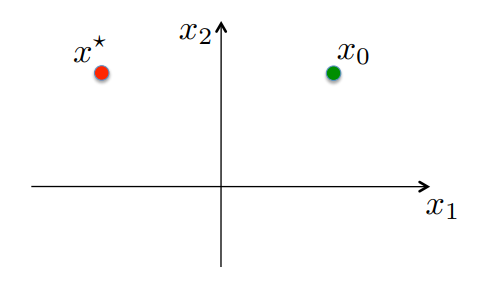
\includegraphics[width=0.5\linewidth]{Bilder/SS1.png}
	\caption{A model for trajectory vs Controllability}
	\label{Fig_2_ch_8_rand1}
\end{figure}
where $x_1$ and $x_2$ are the states for positions and velocities respectively. Notice from figure \ref{Fig_2_ch_8_rand2}, that is not possible to simply go from position  $x$ to $x^{*}$ in this fashion. As by doing so, the state $x_2$ ie., the velocity is either a constant or positive, in both of such cases, it is not possible to move to a negative position by having a positive velocity. Therefore, this trajectory is not possible.
\begin{figure}[h!]
	\centering
	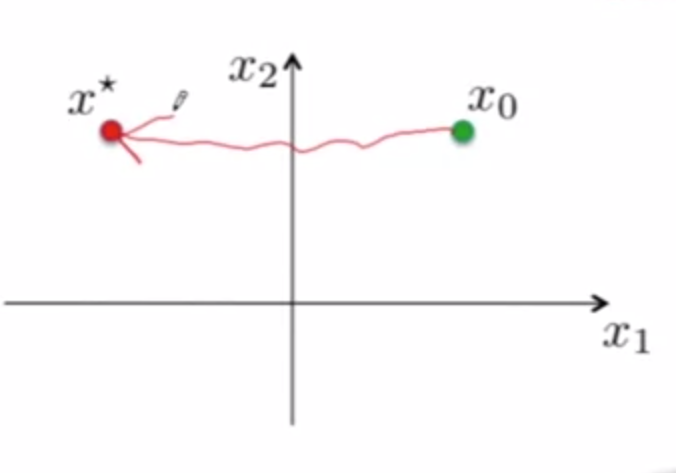
\includegraphics[width=0.5\linewidth]{Bilder/SS2.png}
	\caption{Non possible trajectory}
	\label{Fig_2_ch_8_rand2}
\end{figure}

Further consider, figure \ref{Fig_2_ch_8_rand3}, this would one of the possible trajectories that this system can follow.
\begin{figure}[h!]
	\centering
	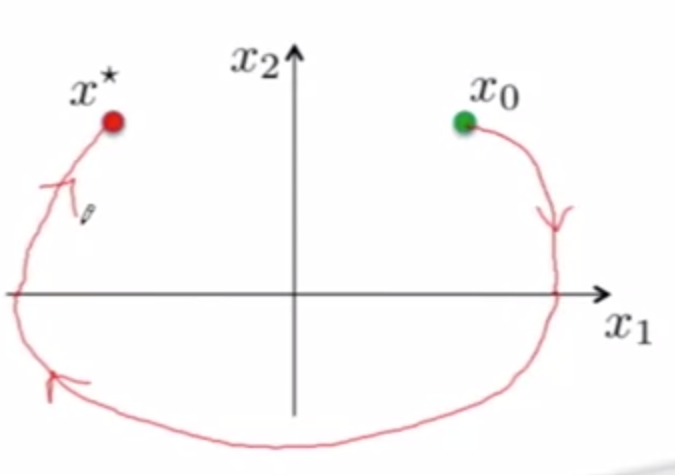
\includegraphics[width=0.5\linewidth]{Bilder/SS3.png}
	\caption{Possible trajectory}
	\label{Fig_2_ch_8_rand3}
\end{figure}